\section{Can a User Notice? (RQ2)}
\label{sec:detection}

A skew that doubles the odds of meeting a narrative changes its share of issue videos from 6.2\% to about 12\%: one more video in every seventeen. Nobody keeps such a count while scrolling. The fair question is whether a tool on the user's side could, given a classifier and a reference feed. \Cref{prop:detect} answers it with a conventional test (level 0.05, power 0.8), and \cref{fig:detection} draws the consequences.

\paragraph{Detecting a doubling takes about \nDetNDouble{} labelled issue videos in each sample.} With the validated classifier of \cref{sec:data} ($\alpha=0.79$, $\beta=0.010$), telling $V=\log 2$ from zero needs \nDetNDouble{} issue videos from the user's feed and as many from the reference; perfect labels would need \nDetNPerfectDouble, a keyword list about \nDetNKeywordDouble. The requirement falls quickly for larger skews (\nDetNHigh{} videos at $V=1.5$) and rises steeply for smaller ones (\nDetNLow{} at $V=0.3$), since it scales with the inverse square of the difference in shares.

\paragraph{The user's own sample is quick to collect; the reference is not.} A topic fan sees about \nIssuePerDayFan{} issue videos a day, so their own \nDetNDouble{} videos accumulate in \nDetDaysFanDouble{} days. The natural reference is the same topic with personalisation switched off. That feed carries the platform's average topic share of 2.4\%, about \nIssuePerDayAvg{} issue videos a day, so the reference sample takes \nDetRefDaysDouble{} days of viewing, close to four months, and \nDetMonthsAvgLow{} months for $V=0.3$ (\cref{fig:detection}b). A user cannot browse two feeds at once for that long. The comparison becomes practical only if the reference is collected once and shared, by a research panel or by the platform itself publishing the non-personalised share of each tracked narrative.

\paragraph{The reference also limits what can be found.} A comparison with the non-personalised feed measures $V_u$ alone. The platform layer $\Lambda$ is common to both samples and cancels (\cref{prop:reach}). Finding it needs the supply share, which only the platform or an outside audit of the catalogue can provide.

\begin{figure}[t]
  \centering
  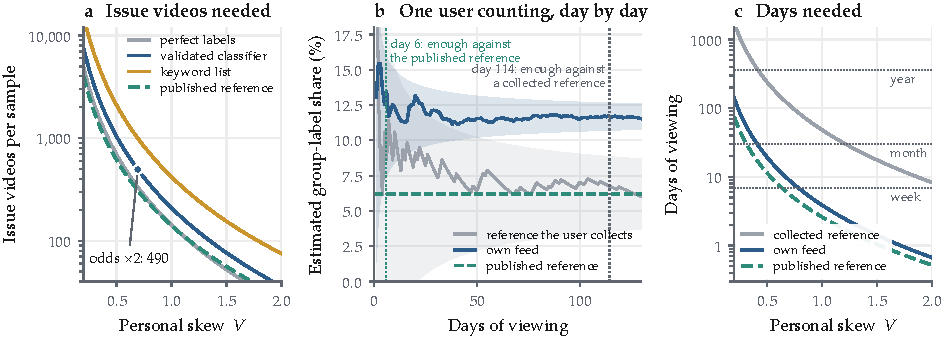
\includegraphics[width=\textwidth]{figures/fig_detection.pdf}
  \caption{What it takes to notice a viewpoint skew. \textbf{(a)} Issue videos needed in each of the two samples (the user's feed and the reference) to detect a personal skew $V$, for three classifiers (\cref{eq:detect}). Dots mark a doubling of the odds and the skew formed in \cref{sec:sim}. \textbf{(b)} Days of viewing needed to collect that many issue videos with the validated classifier: in the feed of a topic fan, and in a reference feed without personalisation.}
  \label{fig:detection}
\end{figure}
